\documentclass[12pt, titlepage]{article}

\usepackage{fullpage}
\usepackage[round]{natbib}
\usepackage{multirow}
\usepackage{booktabs}
\usepackage{tabularx}
\usepackage{graphicx}
\usepackage{float}
\usepackage{hyperref}
\hypersetup{
    colorlinks,
    citecolor=blue,
    filecolor=black,
    linkcolor=red,
    urlcolor=blue
}

%% Comments

\usepackage{color}

\newif\ifcomments\commentstrue %displays comments
%\newif\ifcomments\commentsfalse %so that comments do not display

\ifcomments
\newcommand{\authornote}[3]{\textcolor{#1}{[#3 ---#2]}}
\newcommand{\todo}[1]{\textcolor{red}{[TODO: #1]}}
\else
\newcommand{\authornote}[3]{}
\newcommand{\todo}[1]{}
\fi

\newcommand{\wss}[1]{\authornote{blue}{SS}{#1}} 
\newcommand{\plt}[1]{\authornote{magenta}{TPLT}{#1}} %For explanation of the template
\newcommand{\an}[1]{\authornote{cyan}{Author}{#1}}

%% Common Parts

\newcommand{\progname}{SFWRENG 4G06} % PUT YOUR PROGRAM NAME HERE
\newcommand{\authname}{Team 9, dice\_devs
\\ John Popovici
\\ Nigel Moses
\\ Naishan Guo
\\ Hemraj Bhatt
\\ Isaac Giles} % AUTHOR NAMES                  

\usepackage{hyperref}
    \hypersetup{colorlinks=true, linkcolor=blue, citecolor=blue, filecolor=blue,
                urlcolor=blue, unicode=false}
    \urlstyle{same}
                                


\newcounter{acnum}
\newcommand{\actheacnum}{AC\theacnum}
\newcommand{\acref}[1]{AC\ref{#1}}

\newcounter{ucnum}
\newcommand{\uctheucnum}{UC\theucnum}
\newcommand{\uref}[1]{UC\ref{#1}}

\newcounter{mnum}
\newcommand{\mthemnum}{M\themnum}
\newcommand{\mref}[1]{M\ref{#1}}

\begin{document}

\title{Module Guide for \\\progname: \\Dice Duels: Duel of the Eights} 
\author{\authname}
\date{\today}

\maketitle

\pagenumbering{roman}

\section{Revision History}

\begin{table}[hp]
\caption{Revision History} \label{TblRevisionHistory}
\begin{tabularx}{\textwidth}{llX}
\toprule
\textbf{Date} & \textbf{Developer(s)} & \textbf{Change}\\
\midrule
2025-01-08 & Hemraj Bhatt & Added content to sections 4.1 \& 4.2\\
2025-01-11 & John Popovici & Formatted section 2; Added content to sections 4.1 \& 4.2\\
2025-01-11 & Hemraj Bhatt & Updated content on section 4\\
2025-01-14 & Hemraj Bhatt & Updated content on section 3\\
2025-01-15 & John Popovici & Added content to section 10\\
2025-01-15 & Nigel Moses & Added content to sections 5 \& 10\\
2025-01-16 & Isaac Giles & Added content to sections 6 \& 8\\
2025-01-16 & Hemraj Bhatt & Added content to section 12\\
2025-01-16 & Naishan Guo & Added content to section 9\\
2025-01-17 & John Popovici & Program name and figure 1\\
\bottomrule
\end{tabularx}
\end{table}

\newpage

\section{Reference Material}

This section records information for easy reference.

\subsection{Abbreviations and Acronyms}

\renewcommand{\arraystretch}{1.2}
\begin{tabular}{l l} 
  \toprule		
  \textbf{symbol} & \textbf{description}\\
  \midrule 
  AC & Anticipated Change\\
  M & Module \\
  MG & Module Guide \\
  OS & Operating System \\
  R & Requirement\\
  SC & Scientific Computing \\
  SRS & Software Requirements Specification\\
  \progname & Software Engineering Capstone Course\\
  UC & Unlikely Change \\
  \bottomrule
\end{tabular}\\

See \href{https://github.com/John-Popovici/duel-of-the-eights/blob/main/docs/SRS/SRS.pdf}{SRS Documentation} for any additional.

\newpage

\tableofcontents

\listoftables

\listoffigures

\newpage

\pagenumbering{arabic}

\section{Introduction}
\textbf{Template introduction refactored. A few wording changes.}\\

\noindent{}Decomposing a system into modules is a commonly accepted approach to developing software. A module is a work assignment for a programmer or programming team~\citep{ParnasEtAl1984}. For the Dual of the Eights project, we advocate a decomposition based on the principle of information hiding~\citep{Parnas1972a}. This principle supports design for change, as the "secrets" that each module hides represent likely future changes. This approach is particularly valuable in the context of Dual of the Eights, where modifications to game rules, mechanics, or visual elements are likely during development and playtesting phases.

Our design follows the guidelines laid out by \citet{ParnasEtAl1984}, as follows:
\begin{itemize}
\item System details that are likely to change independently, such as scoring algorithms, dice physics, or player health mechanics, should be the secrets of separate modules.
\item Each data structure, such as those representing dice, players, or game states, is implemented in only one module.
\item Any other module requiring information stored in a module's data structures must obtain it by calling access programs belonging to that module.
\end{itemize}

After completing the first stage of the design, the Software Requirements
Specification (SRS), the Module Guide (MG) is developed~\citep{ParnasEtAl1984}. The MG
specifies the modular structure of the system and is intended to allow both
designers and maintainers to easily identify the parts of the software.  The
potential readers of this document are as follows:

\begin{itemize}
\item New project members: This document can be a guide for a new project member
  to easily understand the overall structure and quickly find the
  relevant modules they are searching for.
\item Maintainers: The hierarchical structure of the module guide improves the
  maintainers' understanding when they need to make changes to the system. It is
  important for a maintainer to update the relevant sections of the document
  after changes have been made.
\item Designers: Once the module guide has been written, it can be used to
  check for consistency, feasibility, and flexibility. Designers can verify the
  system in various ways, such as consistency among modules, feasibility of the
  decomposition, and flexibility of the design.
\end{itemize}

The rest of the document is organized as follows. Section
\ref{SecChange} lists the anticipated and unlikely changes of the software
requirements. Section \ref{SecMH} summarizes the module decomposition that
was constructed according to the likely changes. Section \ref{SecConnection}
specifies the connections between the software requirements and the
modules. Section \ref{SecMD} gives a detailed description of the
modules. Section \ref{SecTM} includes two traceability matrices. One checks
the completeness of the design against the requirements provided in the SRS. The
other shows the relation between anticipated changes and the modules. Section
\ref{SecUse} describes the use relation between modules.

\section{Anticipated and Unlikely Changes} \label{SecChange}

This section lists possible changes to the system. According to the likeliness
of the change, the possible changes are classified into two
categories. Anticipated changes are listed in Section \ref{SecAchange}, and
unlikely changes are listed in Section \ref{SecUchange}.

\subsection{Anticipated Changes} \label{SecAchange}

Anticipated changes are the source of the information that is to be hidden
inside the modules. Ideally, changing one of the anticipated changes will only
require changing the one module that hides the associated decision. The approach
adapted here is called design for
change.

\begin{description}
\item[\refstepcounter{acnum} \actheacnum \label{acOS}:] Operating System: Godot makes porting the game to other operating systems simpler, but specific interfaces may have to change and testing would be required.
\item[\refstepcounter{acnum} \actheacnum \label{acHardware}:] Hardware: The specific hardware on which the software runs is expected to evolve, particularly as the online multiplayer functionality will require a server to enable long-distance gameplay. This aspect of the project is subject to change based on cost, performance, and scalability requirements.
\item[\refstepcounter{acnum} \actheacnum \label{acUserInput}:] User Input: The format of the initial input data is expected to evolve to accommodate users in operating the game and setting game rules. These changes will be made to minimize user errors and facilitate a smoother gameplay experience.
\item[\refstepcounter{acnum} \actheacnum \label{acFileType}:] File Type: The file structure for saving game states and related data is expected to evolve. A file structure that ensures efficient storage and facilitates quick retrieval of game states is expected to be used. 
\item[\refstepcounter{acnum} \actheacnum \label{acScoring}:] Scoring: The scoring calculations may be modified based on usability and player testing.
\item[\refstepcounter{acnum} \actheacnum \label{acUI}:] User Interface (UI): A rudimentary UI is currently used for development. The UI will need to be updated to accommodate the addition of animations and will have to be refreshed in order to look more appealing once the game's major features are complete.
\item[\refstepcounter{acnum} \actheacnum \label{acDice}:] Dice: Dice types can continually be added and modified as they use a simple interface and if added are simple to integrate within the larger system.
\end{description}

% \wss{Anticipated changes relate to changes that would be made in requirements, design or implementation choices.  They are not related to changes that are made at run-time, like the values of parameters.}

\subsection{Unlikely Changes} \label{SecUchange}

The module design should be as general as possible. However, a general system is
more complex. Sometimes this complexity is not necessary. Fixing some design
decisions at the system architecture stage can simplify the software design. If
these decision should later need to be changed, then many parts of the design
will potentially need to be modified. Hence, it is not intended that these
decisions will be changed.

\begin{description}
\item[\refstepcounter{ucnum} \uctheucnum \label{ucInput}:] Input Devices: The game is designed to play on a computer, i.e. it is designed to work with a keyboard and mouse. It is unlikely that the game will be playable through other input means such as controllers.
\item[\refstepcounter{ucnum} \uctheucnum \label{ucOutput}:] Output Devices: The game is designed to play on a computer, i.e. it is designed to display correctly on a computer screen. It is unlikely that the game will be playable through other devices who have vastly different screen sizes such as phones.
\item[\refstepcounter{ucnum} \uctheucnum \label{ucGames}:] Game Types: Despite being likely changes in the SRS stage of development, once formed, the game types designed would require massive module changes if they were to further be modified.
\end{description}

\newpage
\section{Module Hierarchy} \label{SecMH}

This section provides an overview of the module design. Modules are summarized
in a hierarchy decomposed by secrets. The modules listed
below, which are leaves in the hierarchy tree, are the modules that will
actually be implemented.

The modules are categorized into three types: Hardware-Hiding, Behavior-Hiding, and Software Decision modules. Below is the hierarchy:

\subsection{Hardware-Hiding Modules}
\begin{itemize}
    \item \textbf{NetworkManager2P Module:} Manages connection and synchronization for two-player games.
    \item \textbf{GameUI Module:} Provides the interface for interacting with the game and displaying relevant data.
\end{itemize}

\subsection{Behavior-Hiding Modules}
\begin{itemize}
    \item \textbf{MultiGameManager Module:} Manages the sequence of multiple Yahtzee games and customization phases.
    \item \textbf{PlayerManager Module:} Tracks player states, scores, and upgrades.
    \item \textbf{GameManager Module:} Handles a single game of Yahtzee.
    \item \textbf{GameSettings Module:} Loads and stores settings for this Yahtzee variant.
    \item \textbf{CustomizationMenu Module:} Implements dice and game customization between games.
    \item \textbf{DynamicScoreboard Module:} Tracks and displays scores dynamically.
    \item \textbf{CustomBaseDie Module:} Handles the 3D dice models, textures, and physics.
    \item \textbf{DynamicDiceContainer Module:} Manages dice interactions and rendering.
\end{itemize}

\subsection{Software Decision Modules}
\begin{itemize}
    \item \textbf{ScoreCalculator Module:} Calculates scores for dice rolls based on Yahtzee rules and custom modifiers.
\end{itemize}

\section{Connection Between Requirements and Design} \label{SecConnection}

The design of the system is intended to satisfy the requirements developed in
the SRS. In this stage, the system is decomposed into modules. The connection
between requirements and modules is listed in Section 7.

\begin{table}[H]
  \centering
  \resizebox{\textwidth}{!}{
  \begin{tabular}{|l|p{6cm}|p{4cm}|p{5cm}|}
  \hline
  \textbf{Requirement ID} & \textbf{Requirement Description} & \textbf{Module(s) Involved} & \textbf{Design Decision} \\
  \hline
  R1 & Support for online player vs player mode. & NetworkManager2P & Peer-to-peer communication and synchronization are handled by the NetworkManager2P module. \\
  \hline
  R2 & Handle score calculations using Yahtzee rules. & ScoreCalculator & The ScoreCalculator module handles scoring algorithms for standard and non-standard Yahtzee rules. \\
  \hline
  R3 & Simulate realistic physics for 3D dice rolls. & CustomBaseDie, DynamicDiceContainer & Physics for dice rolls are managed by the CustomBaseDie module, and the DynamicDiceContainer deals with dice rendering and states. \\
  \hline
  R4 & Use the real outcome of a roll to get dice values. & CustomBaseDie & The CustomBaseDie module ensures that roll outcomes are derived from physics-based interactions and values are read directly. \\
  \hline
  R5 & Support for dice with different numbers of sides. & CustomBaseDie & The CustomBaseDie module allows updates to dice textures and supports multiple dice variations/configurations. \\
  \hline
  R6 & Implement simultaneous turn-based gameplay. & GameManager, NetworkManager2P & The GameManager controls game flow, while the NetworkManager2P ensures synchronization of simultaneous turns. \\
  \hline
  \end{tabular}}
  \caption{Connection Between Requirements and Modules (Part 1)}
  \label{tab:req_module_connection_part1}
  \end{table}
  
  \begin{table}[H]
  \centering
  \resizebox{\textwidth}{!}{
  \begin{tabular}{|l|p{6cm}|p{4cm}|p{5cm}|}
  \hline
  \textbf{Requirement ID} & \textbf{Requirement Description} & \textbf{Module(s) Involved} & \textbf{Design Decision} \\
  \hline
  R7 & Allow players to pick and omit dice for each roll. & GameManager, DynamicDiceContainer & The GameManager tracks player decisions, and the DynamicDiceContainer updates dice states accordingly. \\
  \hline
  R8 & Display a user interface with scores, dice states, and player information. & GameUI, DynamicScoreboard & The GameUI presents game information, while the DynamicScoreboard provides real-time score updates. \\
  \hline
  R9 & Provide controls for modifying game settings. & GameSettings, CustomizationMenu & The GameSettings module stores configurations, and the CustomizationMenu allows changes to these configurations. \\
  \hline
  R10 & Provide presets for different game modes. & GameSettings & Presets are stored and retrieved through the GameSettings module. \\
  \hline
  R17 & Always show the correct current state accurately. & GameUI, GameManager & State synchronization is managed by the GameManager, while GameUI reflects the current state. \\
  \hline
  NFR2 & Implement a clear and easy-to-use interface. & GameUI & The GameUI module prioritizes usability through intuitive design. \\
  \hline
  NFR6 & Ensure modular, easily extendable codebase. & All Modules & Modular decomposition of functionality ensures extensibility and maintainability. \\
  \hline
  NFR9 & Maintain a consistent UI and 3D visual style. & GameUI, DynamicDiceContainer & Style guidelines and visual coherence are maintained across all UI and gameplay elements. \\
  \hline
  \end{tabular}}
  \caption{Connection Between Requirements and Modules (Part 2)}
  \label{tab:req_module_connection_part2}
  \end{table}


\section{Module Decomposition} \label{SecMD}

Modules are decomposed according to the principle of ``information hiding''
proposed by \citet{ParnasEtAl1984}. The \emph{Secrets} field in a module
decomposition is a brief statement of the design decision hidden by the
module. The \emph{Services} field specifies \emph{what} the module will do
without documenting \emph{how} to do it. For each module, a suggestion for the
implementing software is given under the \emph{Implemented By} title. If the
entry is \emph{OS}, this means that the module is provided by the operating
system or by standard programming language libraries.  \emph{\textit{Dice Duels: Duel of the Eights}} means the
module will be implemented by the \textit{Dice Duels: Duel of the Eights} software.

\subsection{Hardware-Hiding Modules}
The Hardware-Hiding Modules provide an abstraction layer between the system's hardware-dependent functionalities and the rest of the software. These modules ensure that the game interacts efficiently with network communication protocols, rendering processes, and user interface elements. By encapsulating these low-level implementations, other modules can remain independent of platform-specific changes and focus solely on gameplay logic.
\subsubsection{NetworkManager2P Module}
\textbf{Secrets:} The underlying implementation of peer-to-peer communication and synchronization between two clients.\\
\textbf{Services:} Handles connection setup, data synchronization, and disconnection handling for a 2-player game.\\
\textbf{Implemented By:} \textit{Dice Duels: Duel of the Eights}

\subsubsection{GameUI Module}
\textbf{Secrets:} The logic for UI components and interactions.\\
\textbf{Services:} Displays information to players, including scores and customization options, and provides action buttons.\\
\textbf{Implemented By:} \textit{Dice Duels: Duel of the Eights}

\subsection{Behavior-Hiding Modules}
The Behavior-Hiding Modules define the core functionality and game flow in Dice Duels. These modules are responsible for handling game management, player state tracking, customization systems, and dynamic score calculations. By isolating gameplay mechanics from low-level interactions, these modules ensure flexibility, scalability, and ease of modification without impacting the underlying hardware or system-dependent components.
\subsubsection{MultiGameManager Module}
\textbf{Secrets:} The logic for managing multiple games, including customization and upgrades between games.\\
\textbf{Services:} Tracks progress and integrates player upgrades into gameplay.\\
\textbf{Implemented By:} \textit{Dice Duels: Duel of the Eights}

\subsubsection{PlayerManager Module}
\textbf{Secrets:} The data structure for tracking player-specific details, including scores, dice, and upgrades.\\
\textbf{Services:} Tracks and updates player states, including consumables and modifiers.\\
\textbf{Implemented By:} \textit{Dice Duels: Duel of the Eights}

\subsubsection{GameManager Module}
\textbf{Secrets:} The logic for managing the flow of the game.\\
\textbf{Services:} Tracks game progress and controls flow and state of the game.\\
\textbf{Implemented By:} \textit{Dice Duels: Duel of the Eights}

\subsubsection{GameSettings Module}
\textbf{Secrets:} Configuration storage and retrieval.\\
\textbf{Services:} Stores and loads game settings, including the number of games and customization options.\\
\textbf{Implemented By:} \textit{Dice Duels: Duel of the Eights}

\subsubsection{CustomizationMenu Module}
\textbf{Secrets:} The logic for presenting and applying customization options between games.\\
\textbf{Services:} Displays upgrade options, enforces selection rules, and updates player dice and modifiers.\\
\textbf{Implemented By:} \textit{Dice Duels: Duel of the Eights}

\subsubsection{DynamicScoreboard Module}
\textbf{Secrets:} The algorithms for dynamically generating score displays.\\
\textbf{Services:} Updates and displays scores in real-time during gameplay.\\
\textbf{Implemented By:} \textit{Dice Duels: Duel of the Eights}

\subsubsection{CustomBaseDie Module}
\textbf{Secrets:} The interaction logic and rendering of custom dice, including dynamic face changes.\\
\textbf{Services:} Manages dice texture changes based on player customization and handles physics and collision for rolling.\\
\textbf{Implemented By:} \textit{Dice Duels: Duel of the Eights}

\subsubsection{DynamicDiceContainer Module}
\textbf{Secrets:} The algorithms for managing a collection of dice and their rendering.\\
\textbf{Services:} Dynamically creates and organizes dice based on game settings and updates dice states during gameplay.\\
\textbf{Implemented By:} \textit{Dice Duels: Duel of the Eights}

\subsection{Software Decision Modules}
The Software Decision Modules contain mathematical and algorithmic implementations that are not explicitly outlined in the system's specifications but are essential for achieving key functionalities. These modules include scoring calculations and rule enforcement, ensuring accurate scorekeeping and rule adherence throughout the game. These components work independently of user interaction but provide crucial support for the game logic.
\subsubsection{ScoreCalculator Module}
\textbf{Secrets:} The scoring algorithms based on Yahtzee rules and custom modifiers.\\
\textbf{Services:} Calculates scores for dice rolls and applies passive modifiers.\\
\textbf{Implemented By:} \textit{Dice Duels: Duel of the Eights}





\newpage
\section{Traceability Matrix} \label{SecTM}

This section shows two traceability matrices: between the modules and the
requirements and between the modules and the anticipated changes.

\begin{table}[H]
  \centering
  \begin{tabular}{p{0.2\textwidth} p{0.6\textwidth}}
  \toprule
  \textbf{Req.} & \textbf{Modules}\\
  \midrule
  R1 & NetworkManager2P, GameManager\\
  R2 & ScoreCalculator\\
  R3 & CustomBaseDie, DynamicDiceContainer\\
  R4 & CustomBaseDie\\
  R5 & CustomBaseDie\\
  R6 & GameManager, NetworkManager2P\\
  R7 & GameManager, DynamicDiceContainer\\
  R8 & GameUI, DynamicScoreboard\\
  R9 & GameSettings, CustomizationMenu\\
  R10 & GameSettings\\
  R17 & GameManager, GameUI\\
  \bottomrule
  \end{tabular}
  \caption{Trace Between Requirements and Modules}
  \label{TblRT}
  \end{table}
  
  \begin{table}[H]
  \centering
  \begin{tabular}{p{0.2\textwidth} p{0.6\textwidth}}
  \toprule
  \textbf{AC} & \textbf{Modules}\\
  \midrule
  AC1 & GameUI, NetworkManager2P\\
  AC2 & NetworkManager2P\\
  AC3 & GameUI, GameSettings\\
  AC4 & GameManager, GameSettings\\
  AC5 & ScoreCalculator\\
  AC6 & GameUI\\
  AC7 & CustomBaseDie, DynamicDiceContainer\\
  \bottomrule
  \end{tabular}
  \caption{Trace Between Anticipated Changes and Modules}
  \label{TblACT}
  \end{table}

\newpage
\section{Use Hierarchy Between Modules} \label{SecUse}

In this section, the uses hierarchy between modules is
provided. \citet{Parnas1978} said of two programs A and B that A {\em uses} B if
correct execution of B may be necessary for A to complete the task described in
its specification. That is, A {\em uses} B if there exist situations in which
the correct functioning of A depends upon the availability of a correct
implementation of B.  Figure \ref{FigUH} illustrates the use relation between
the modules. It can be seen that the graph is a directed acyclic graph
(DAG). Each level of the hierarchy offers a testable and usable subset of the
system, and modules in the higher level of the hierarchy are essentially simpler
because they use modules from the lower levels.



\begin{figure}[H]
\centering
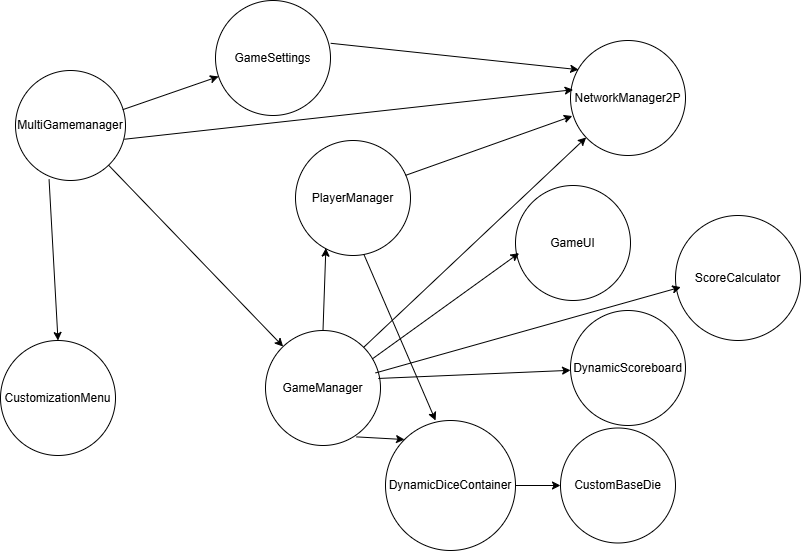
\includegraphics[width=0.8\textwidth]{figures/UsesHierarchy}
\caption{Use hierarchy among modules}
\label{FigUH}
\end{figure}

%\section*{References}

\newpage
\section{User Interfaces}

% \wss{Design of user interface for software and hardware.  Attach an appendix if needed. Drawings, Sketches, Figma}

%%%%%%%%%%%%%%%%%%%%%%%%%%%%%%%%%%%%%%%%%%%%%%%%%%%%%%%%%%%%%%%%%%%%%
\begin{figure}[h!]
\caption{Main Menu User Interface Sketch}
\centering

\includegraphics[width=0.9\textwidth]{figures/main_menu}
\end{figure}



%%%%%%%%%%%%%%%%%%%%%%%%%%%%%%%%%%%%%%%%%%%%%%%%%%%%%%%%%%%%%%%%%%%%%
\begin{figure}[h!]
\caption{Settings Menu User Interface Sketch}
\centering
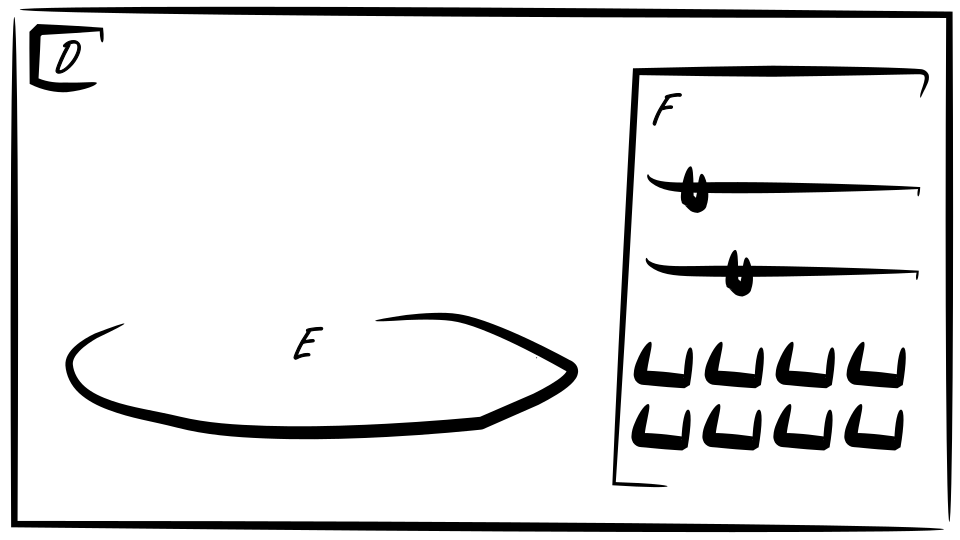
\includegraphics[width=0.9\textwidth]{figures/settings}
\end{figure}



%%%%%%%%%%%%%%%%%%%%%%%%%%%%%%%%%%%%%%%%%%%%%%%%%%%%%%%%%%%%%%%%%%%%%
\begin{figure}[h!]
\caption{Game User Interface Sketch}
\centering
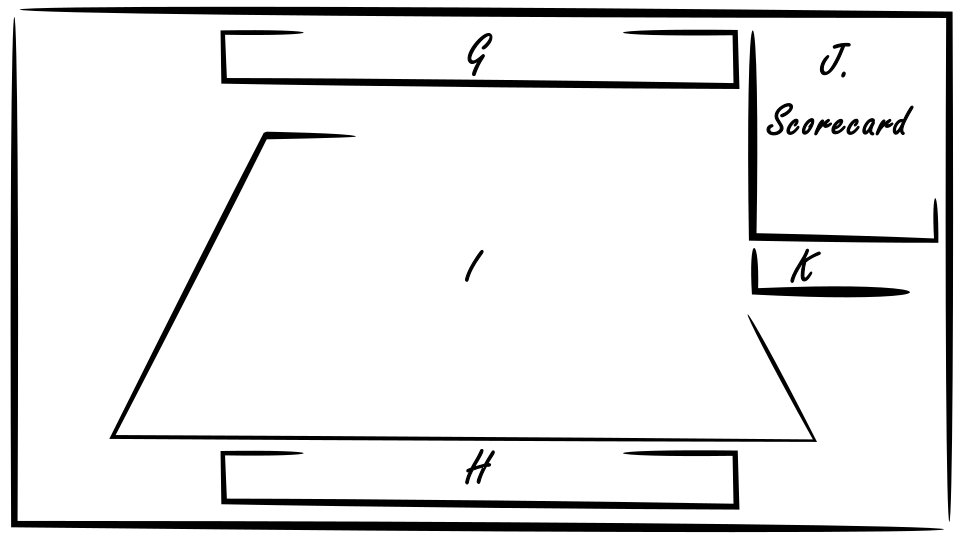
\includegraphics[width=0.9\textwidth]{figures/game_interface}
\end{figure}



%%%%%%%%%%%%%%%%%%%%%%%%%%%%%%%%%%%%%%%%%%%%%%%%%%%%%%%%%%%%%%%%%%%%%
\begin{figure}[h!]
\caption{Game Creation User Interface Sketch}
\centering
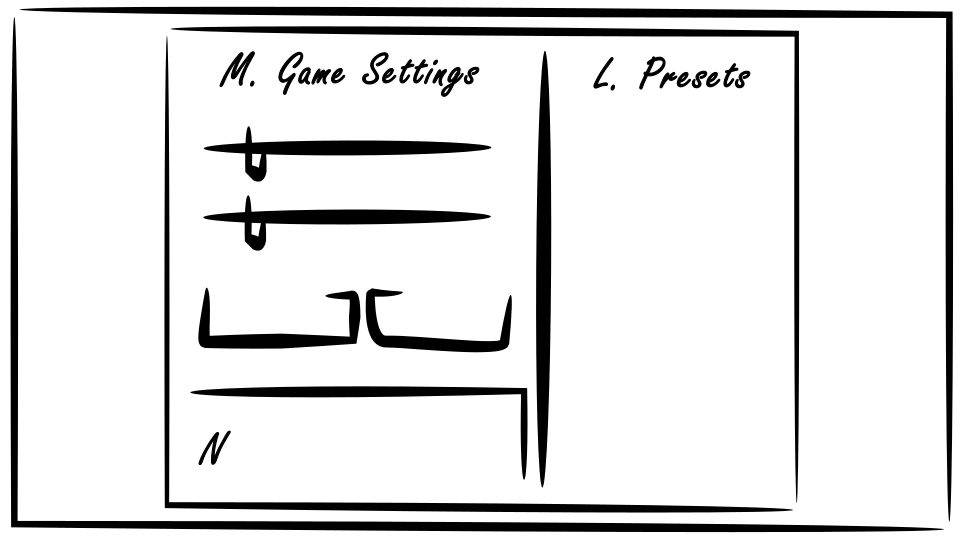
\includegraphics[width=0.9\textwidth]{figures/game_creation}
\end{figure}



~
\newpage
~
\newpage

\noindent
Elements of the main menu user interface:
\begin{itemize}
  \item A: Title and game name
  \item B: Menu and game options
  \item C: Options and settings
\end{itemize}
Elements of the settings menu user interface:
\begin{itemize}
  \item D: Back to main menu
  \item E: Dice example display
  \item F: Customization options
\end{itemize}
Elements of the game user interface:
\begin{itemize}
  \item G: Opponent display dice information
  \item H: Player display dice information
  \item I: Game board display
  \item J: Scorecard and score
  \item K: Game turn controls
\end{itemize}
Elements of the game creation user interface:
\begin{itemize}
  \item L: Game presets controls
  \item M: Customizable game settings
  \item N: Game connection and start information
\end{itemize}









~\newpage
\section{Design of Communication Protocols}

The communication protocols for this project leverage Godot's built-in multiplayer networking libraries to facilitate data synchronization and interactions between players. The design supports two key modes of communication: local area network (LAN) and online multiplayer through a server-based hosting system.

\subsection{Use of Godot Multiplayer Networking Libraries}

Godot's multiplayer networking system provides the foundation for real-time communication between players. The networking stack includes:
\begin{itemize}
    \item \textbf{ENet Protocol:} A reliable UDP-based protocol for efficient and low-latency data transmission.
    \item \textbf{@rpc and @rpc("any\_peer") Functions:} Remote Procedure Calls (RPCs) are used to synchronize state and transmit data between connected peers. The \texttt{@rpc} and \texttt{@rpc("any\_peer")} functions allow for targeted and efficient communication.
\end{itemize}

The networking manager (`networkManager2P`) is designed to handle peer-to-peer communication for two players over a LAN or via an online server. The system uses a host-client architecture, where the host player is responsible for maintaining the game state and transmitting updates to connected clients.

\subsection{Server-Based Hosting for Online Multiplayer}

For online multiplayer, a server will be implemented to host game lobbies for players who are not on the same network. The server's responsibilities include:
\begin{itemize}
    \item Managing multiple lobbies and connections simultaneously.
    \item Authenticating and assigning unique identifiers to each connected player.
    \item Relaying data between the host and clients, ensuring seamless communication.
\end{itemize}

This server-based approach allows players from different locations to connect and ensures a consistent experience by maintaining a central point of synchronization for game state.

\subsection{Types of Data Passed Between Players}

The communication protocol is designed to handle various types of data to synchronize game state and ensure fair gameplay. Based on the `networkManager2P` module, the following types of data are transmitted:
\begin{itemize}
    \item \textbf{Game State Updates:} Includes information about the current round, dice rolls, and scores. These updates ensure both players are in sync at all times.
    \item \textbf{Player Actions:} Data related to specific player interactions, such as dice selections, re-rolls, and scoring decisions.
    \item \textbf{Customization Choices:} Information about selected customizations, such as dice face changes, passive modifiers, and consumables.
    \item \textbf{Connection Management:} Includes data for handling player connections and disconnections. This ensures smooth transitions when players join or leave a game.
\end{itemize}

\subsection{Functions for Data Communication}

The following functions from the `networkManager2P` module facilitate communication:
\begin{itemize}
    \item \texttt{broadcast\_disconnect(state: String, data: Dictionary)}: Calls the rpc receive\_disconnect on peers to notify.
    \item \texttt{receive\_disconnect()}: The rpc function that can be calls to receive a disconnect notification.
    \item \texttt{broadcast\_game\_state(state: String, data: Dictionary)}: Calls the rpc receive\_game\_state on peer to notify each other of game their state.
    \item \texttt{receive\_game\_state(state: String, data: Dictionary)}: The rpc function that is called to receive the other peer's game state.
    \item \texttt{ping()}: Calls itself on all connected peers to track connection status.
    \item \texttt{send\_game\_settings(\_game\_settings: Dictionary,\_hand\_settings: Dictionary)}: Calls the rpc receive\_game\_settings on peer to send the game settings to the client device.
    \item \texttt{receive\_game\_settings(\_game\_settings: Dictionary, \_hand\_settings: Dictionary)}: The rpc function that receives the game settings from the host device.
\end{itemize}

\subsection{Design Considerations}

The communication protocols are designed with the following considerations:
\begin{itemize}
    \item \textbf{Reliability:} The ENet protocol ensures that all critical game state data is reliably delivered to connected peers.
    \item \textbf{Low Latency:} The use of UDP minimizes delays, ensuring real-time synchronization during gameplay.
    \item \textbf{Scalability:} While the current implementation supports two-player games, the architecture can be extended to handle larger multiplayer games if required.
\end{itemize}

This protocol design ensures a robust and flexible communication system for the Yahtzee game, providing a seamless multiplayer experience across both LAN and online environments.


\section{Timeline}

A Gantt chart was created to effectively assign work on modules to team members. The chart can be accessed using the link below:\\

\href{https://mcmasteru365-my.sharepoint.com/:x:/r/personal/bhatth14_mcmaster_ca/Documents/Rev0%20Gnatt%20Chart.xlsx?d=w7c7c84af07004c328dc311a8721a5adb&csf=1&web=1&e=d8G3hJ}{Access Gantt chart}

\bibliographystyle {plainnat}
\bibliography{../../../refs/References}

\newpage{}

\end{document}